% This file (dissertation-main.tex) is the main file for a dissertation.
\documentclass {udthesis}
% preamble

% Include graphicx package for the example image used
% Use LaTeX->PDF if including graphics such as .jpg, .png or .pdf.
% Use LaTeX->PS->PDF if including graphics such as .ps or .eps
% Best practice to not specify the file extension for included images,
% so when LaTeX is building it will look for the appropriate image type.
\usepackage{graphicx}
\usepackage[acronym]{glossaries}
\usepackage{enumitem}
\usepackage{amsmath}
\usepackage{subfigure}
\usepackage{url}

\newacronym{auv}{AUV}{Autonomous Underwater Vehicle}
\newacronym{rov}{ROV}{Remotely Operated Vehicle}
\newacronym{hov}{HOV}{Human Operated Vehicle}
\newacronym{api}{API}{Application Program Interface}
\newacronym{dyi}{DYI}{Do It Yourself}
\newacronym{ros}{ROS}{Robot Operating System}
\newacronym{dof}{DOF}{Degree of Freedom}

\makeglossaries
\graphicspath{{fig/}}

\begin{document}

%=========================================================================================
% CoopROV section

\chapter{CoopROV: Low cost underwater remotely operated vehicle}


%=========================================================================================
% Outline
\section{Outline}

The developed multi-image object recognition theory can be validated using an easily accessible 
open-source robot.

\begin{enumerate}[label=Section \arabic*:, start=0]
\item Intro

\item Commercially available underwater robots are expensive and provide limited flexiblity for incorporation of new sensors and custom controllers.

\item CoopROV based off of the open-source underwater platform openROV, marries the low cost hardware design with seamless integration to ROS for easy application development.

\item An underwater experimental setup in a water tank was designed to collect underwater image data.

\item IMU, depth sensor, stereo camera and AR Tags were used to localize CoopROV.

\item The multi-image object recognition approach was validated using image data gathered from CoopROV.

\end{enumerate}

%========================================================================================

\section{Introduction}

Field experiments related to underwater object recognition require a submersible robot with appropriate sensing and control apparatus to navigate through points of interest and capture necessary data through sensors. Based on level of manual intervention involved to guide the vehicle, there are three main classes of underwater vehicles namely \gls{auv}, \gls{rov} and \gls{hov}. \gls{auv}s navigate autonmously with minimal to no manual support. Both \gls{rov}s and \gls{hov}s are piloted by humans, with the difference that the human operator is within the vehicle in an \gls{hov} whereas in the \gls{rov}, the human operator controls the vehicle from a remote location like a surface vessel. The commercially available underwater vehicles come with wide range of capabilities in terms of sensing and operational depths. The sensing package or the type of vehicle required is dictated by the objective of the science experiment and its requirements. For validation and fine-tuning of the object recognition theory, like 
the multi-layered scallop recognition \ref{chap:scallop_recog} and the multi-image object recognition \ref{chap:distance_des} developed in this thesis, an underwater vehicle that can navigate to specific points and collect image data of underwater target is helpful. With these requirement in mind, a low-cost underwater research vehicle CoopROV was developed. CoopROV is an \gls{rov} class vehicle that comes with several sensors for data collection and also the capability to incorporate any customized controller.

\section{Commercial Submersible Robots}

Commercially available robots are expensive and often provide minimal access to their legacy controllers and software. Most commercial \gls{rov}s come with a graphical interface and joystick to drive the robot. \gls{auv}s come with an interface to allow the user to predefine the robot trajectory through a series of geo-tagged waypoints before deployment. Once deployed, the \gls{auv} tracks the specified trajectory. Such manufacturer interfaces do not provide considerable freedom to modify the core software running the robot. For instance if someone wants to use their own controller, it becomes problematic to implement it without manufacturer supported software \gls{api}s. Cost is another factor that limits access to commercial robots. A relatively small \gls{rov} like the videoray \cite{videoray} with a footprint of $14.75\times 11.4\times 8.75 \,(L\times W\times H \text{ in inches})$ and a sensor package comprising a video camera, gyros, accelerometers, compass, depth and temperature sensors can cost upwards of 25\,000 dollars. Bigger \gls{rov}s like the Outland ROV\cite{outlandrov} can cost upwards of 75\,000 dollars with the cost here being chiefly determined by the sophistication of the on board sensing capabilities. Despite the high cost and minimal flexibity for customer modifications, the primary advantage of these commercial solutions is their well tested hardware that is resilient to harsh conditions that are characteristic to the marine environment.

The other league of underwater robotic solutions come in form of low-cost \gls{dyi} style robots like the OpenROV \cite{openrov} and the Fathom One\cite{fathomrov}. Such solutions offer a lot of potential for custom harware and software modifications. However being small-scale development projects, the associated hardware in these cases are not well tested and are prone to issues like water leaks. The capability of these systems to withstand the harsh conditions of a marine environment is questionable. In terms of software, the source code is often available and comes with an open-source license as in the case of OpenROV. However OpenROV's software does not come with APIs to encourage users to extend or modify the capabilities of the robot. Additionally, the limited documentation available for OpenROV makes the task of directly modifying the source code cumbersome. Since the focus of most of these \gls{dyi} projects are to offer low-cost options that enable hobbyists to explore underwater, a teleoperation interface and access to the camera feed from the robot completes the scope of these projects. For researchers that have very specialized interests, an ideal robotic solution should offer finer control of the harware and software with options to easily extend the base capabilities of the system.

There are two primary requirements for a research robotic solution. The first is the need for a tough exterior shell that can hold up against high values of water pressure which is common with deep sea operation. This exterior shell should also be resilient to water leaks and at the same time offer the ability to retrofit sensors. The second requirement is for the robotic system to offer a well built software interface with \gls{api}s that allows researchers to extend the capabilities of the system to match their needs. It will be beneficial if the software \gls{api}s confirm to popular robotics research architectures like \gls{ros} \cite{ros}. A robot with \gls{ros}-support will greatly enhances the usability of the robot by opening access to a plethora of existing software tools. Furthermore, linking the software with open-source tools like \gls{ros} comes with an active base of researchers for support and scientific discussions. Currently the underwater research community lacks a low-cost submersible robotic platform with resilient hardware design and well engineered software.

\section{CoopROV}

The chief requirements that lead to the design of CoopROV is the need for a low-cost submersible robotic platform that acts as testbed for computer vision and control algorithms. Before the decision to build CoopROV, the existing solutions were evaluated. The commercial robotic solutions like Videoray were clearly outside the price range. OpenROV 2.5 \cite{openrov}, the first version of OpenROV was a good candidate primarily due to it sub-1000 dollar price tag. However multiple tests revealed that the water proofing and electronics had several glitches which made it unsuitable for deployment. These experiments provided useful insights into the core components and associated problems that need to be tackled to design a submersible robot. The original OpenROV design came with a beaglebone and browser based graphical user interface that used node.js \cite{nodejs} in the backend to drive the robot. Most of the algorithm development till that point was in \gls{ros}, hence \gls{ros} support was one of the preffered requirements for the envisioned submersible robot. The design of CoopROV was initiated to address the shortcomings of OpenROVs hardware in terms of waterproofing and electronics. The additional features of the target design was to allow easy interfacing of new sensors along with full \gls{ros} software support for sensors and actuators.

In the current stage of development, CoopROV shows some resemblence to OpenROV as both of them share the same frame and actuators. All electronics, power-supply and sensors in CoopROV have diverged completely from OpenROV 2.5. Two views of CoopROV a frontal view and its the appearance when deployed in a test tank is shown in Figure~\ref{fig:cooprov}.
%
\begin{figure} \label{fig:cooprov}
\centering
\subfigure[]{
      \label{fig:cooprov_front}
      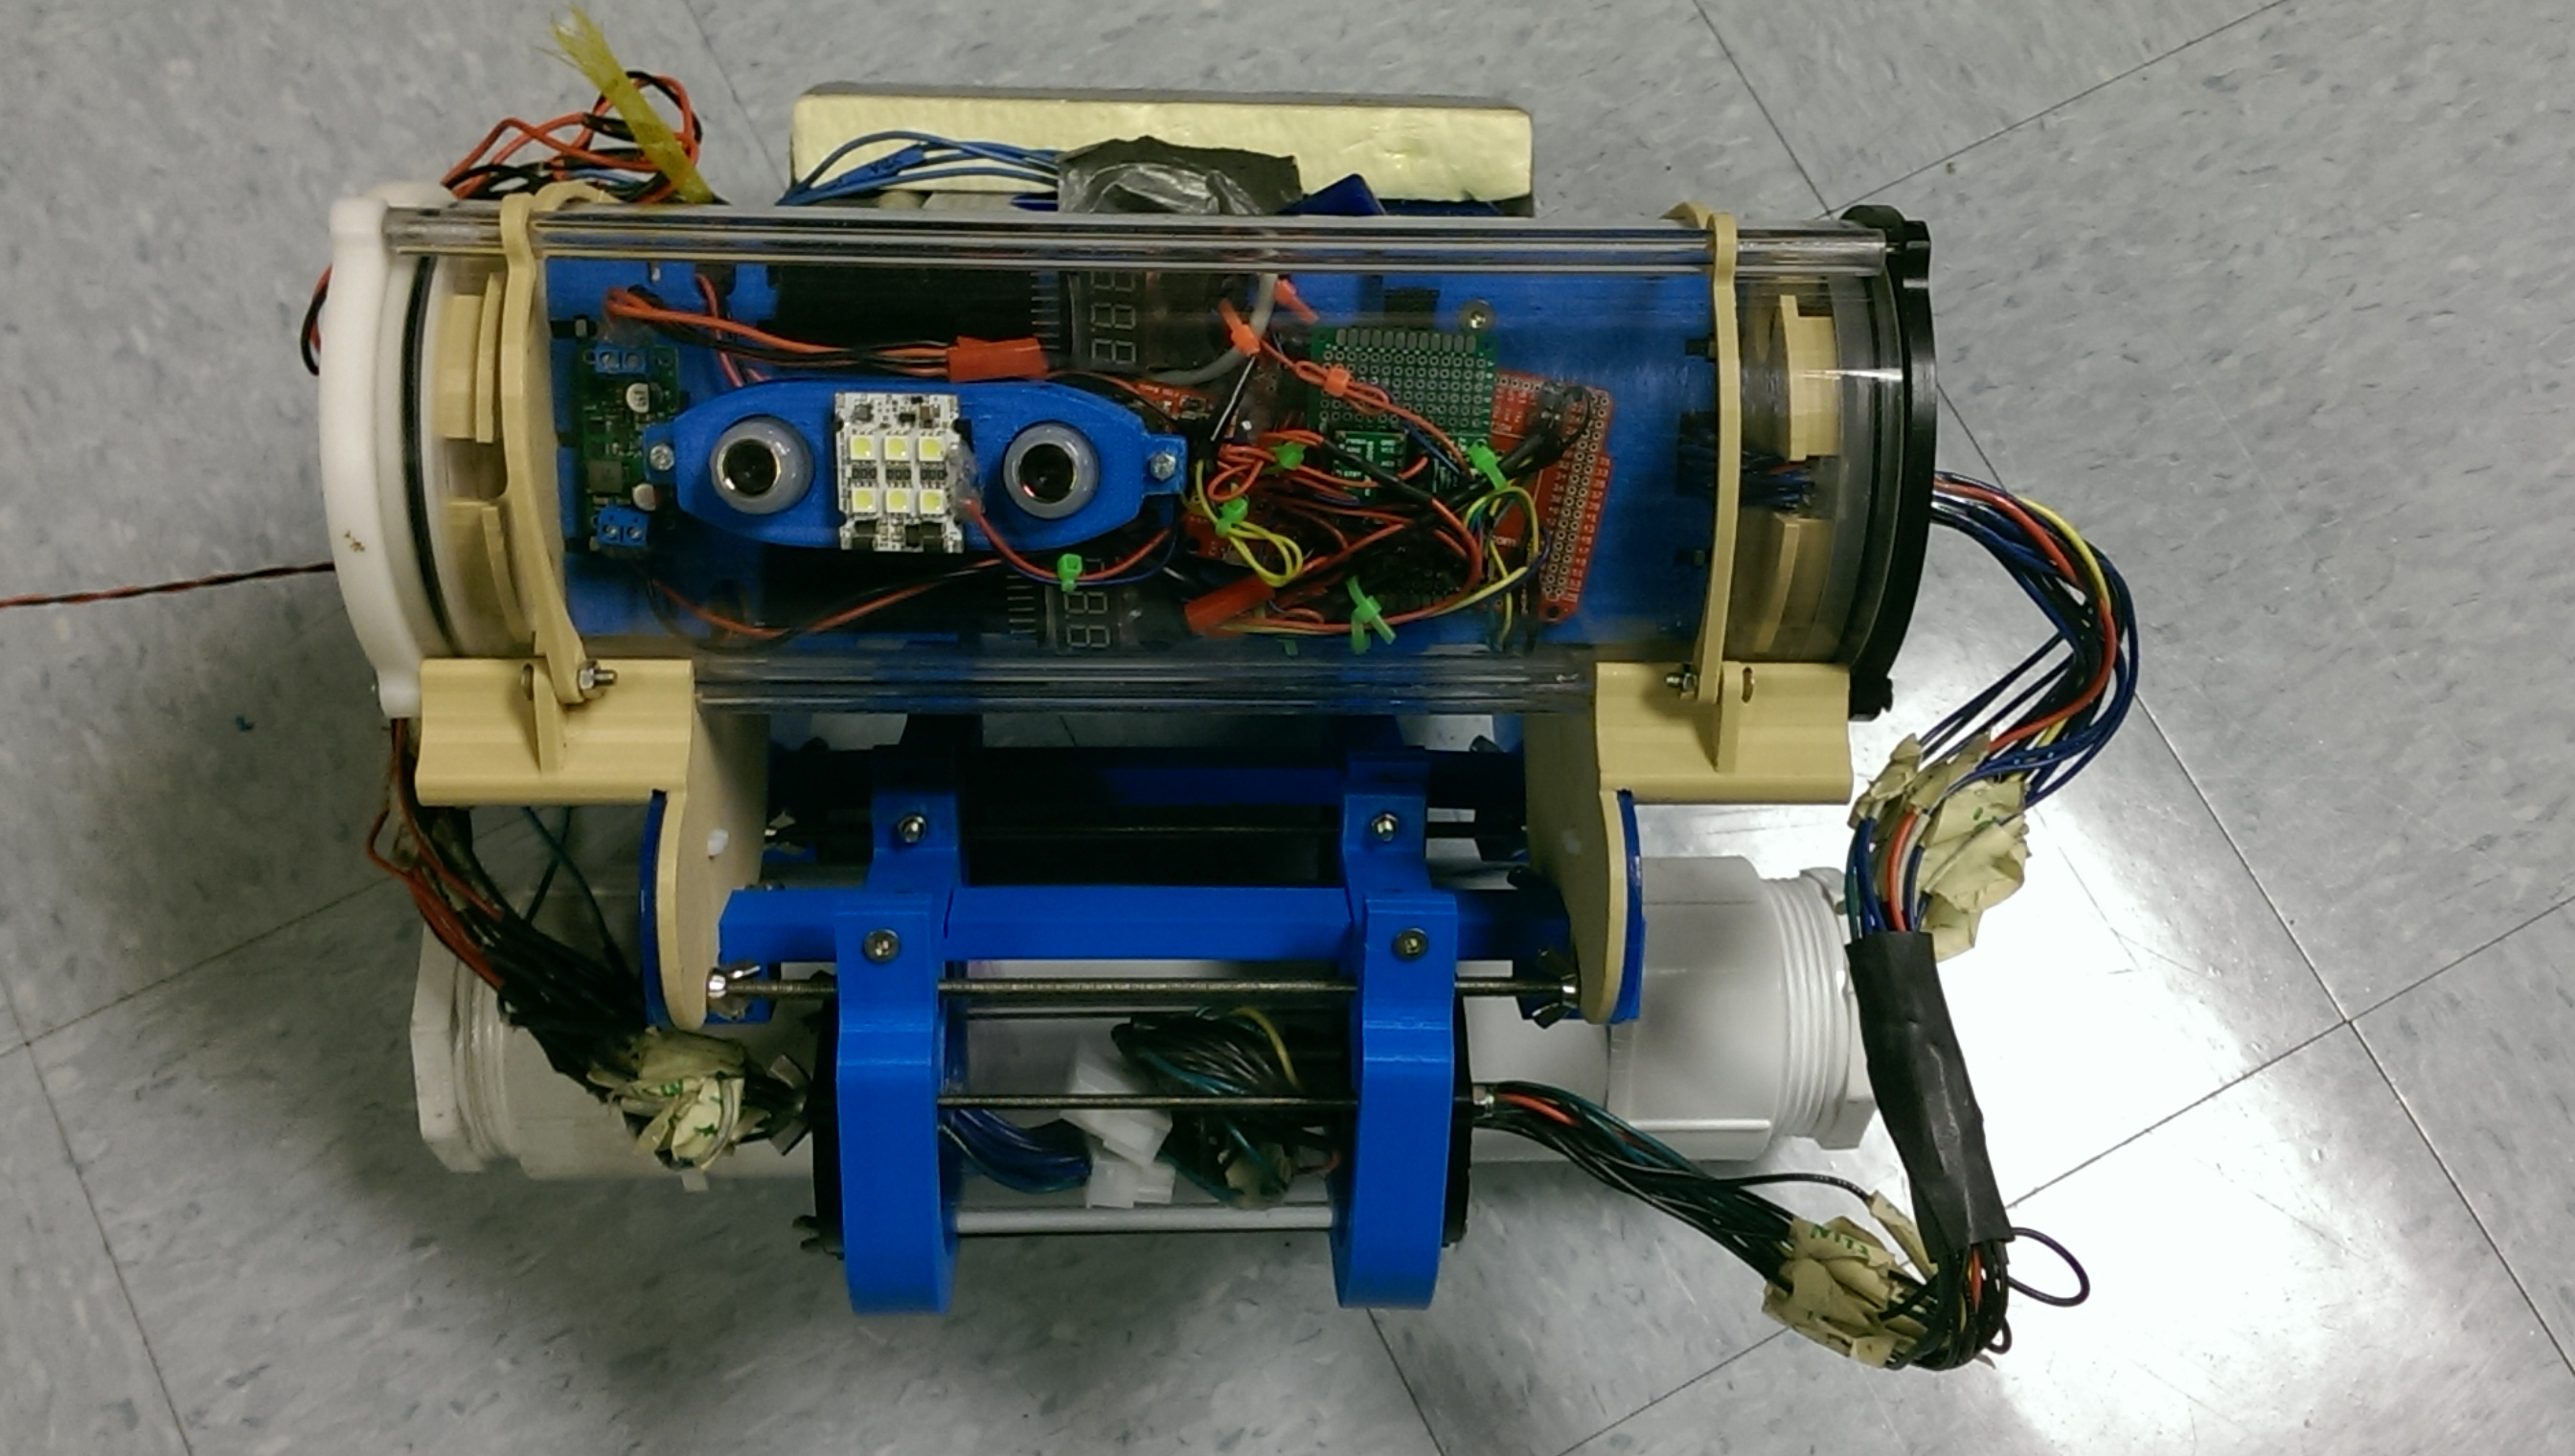
\includegraphics[width=0.45\textwidth]{cooprov_front.jpg}
      }
\subfigure[]{
      \label{subfig:cooprov_top}
      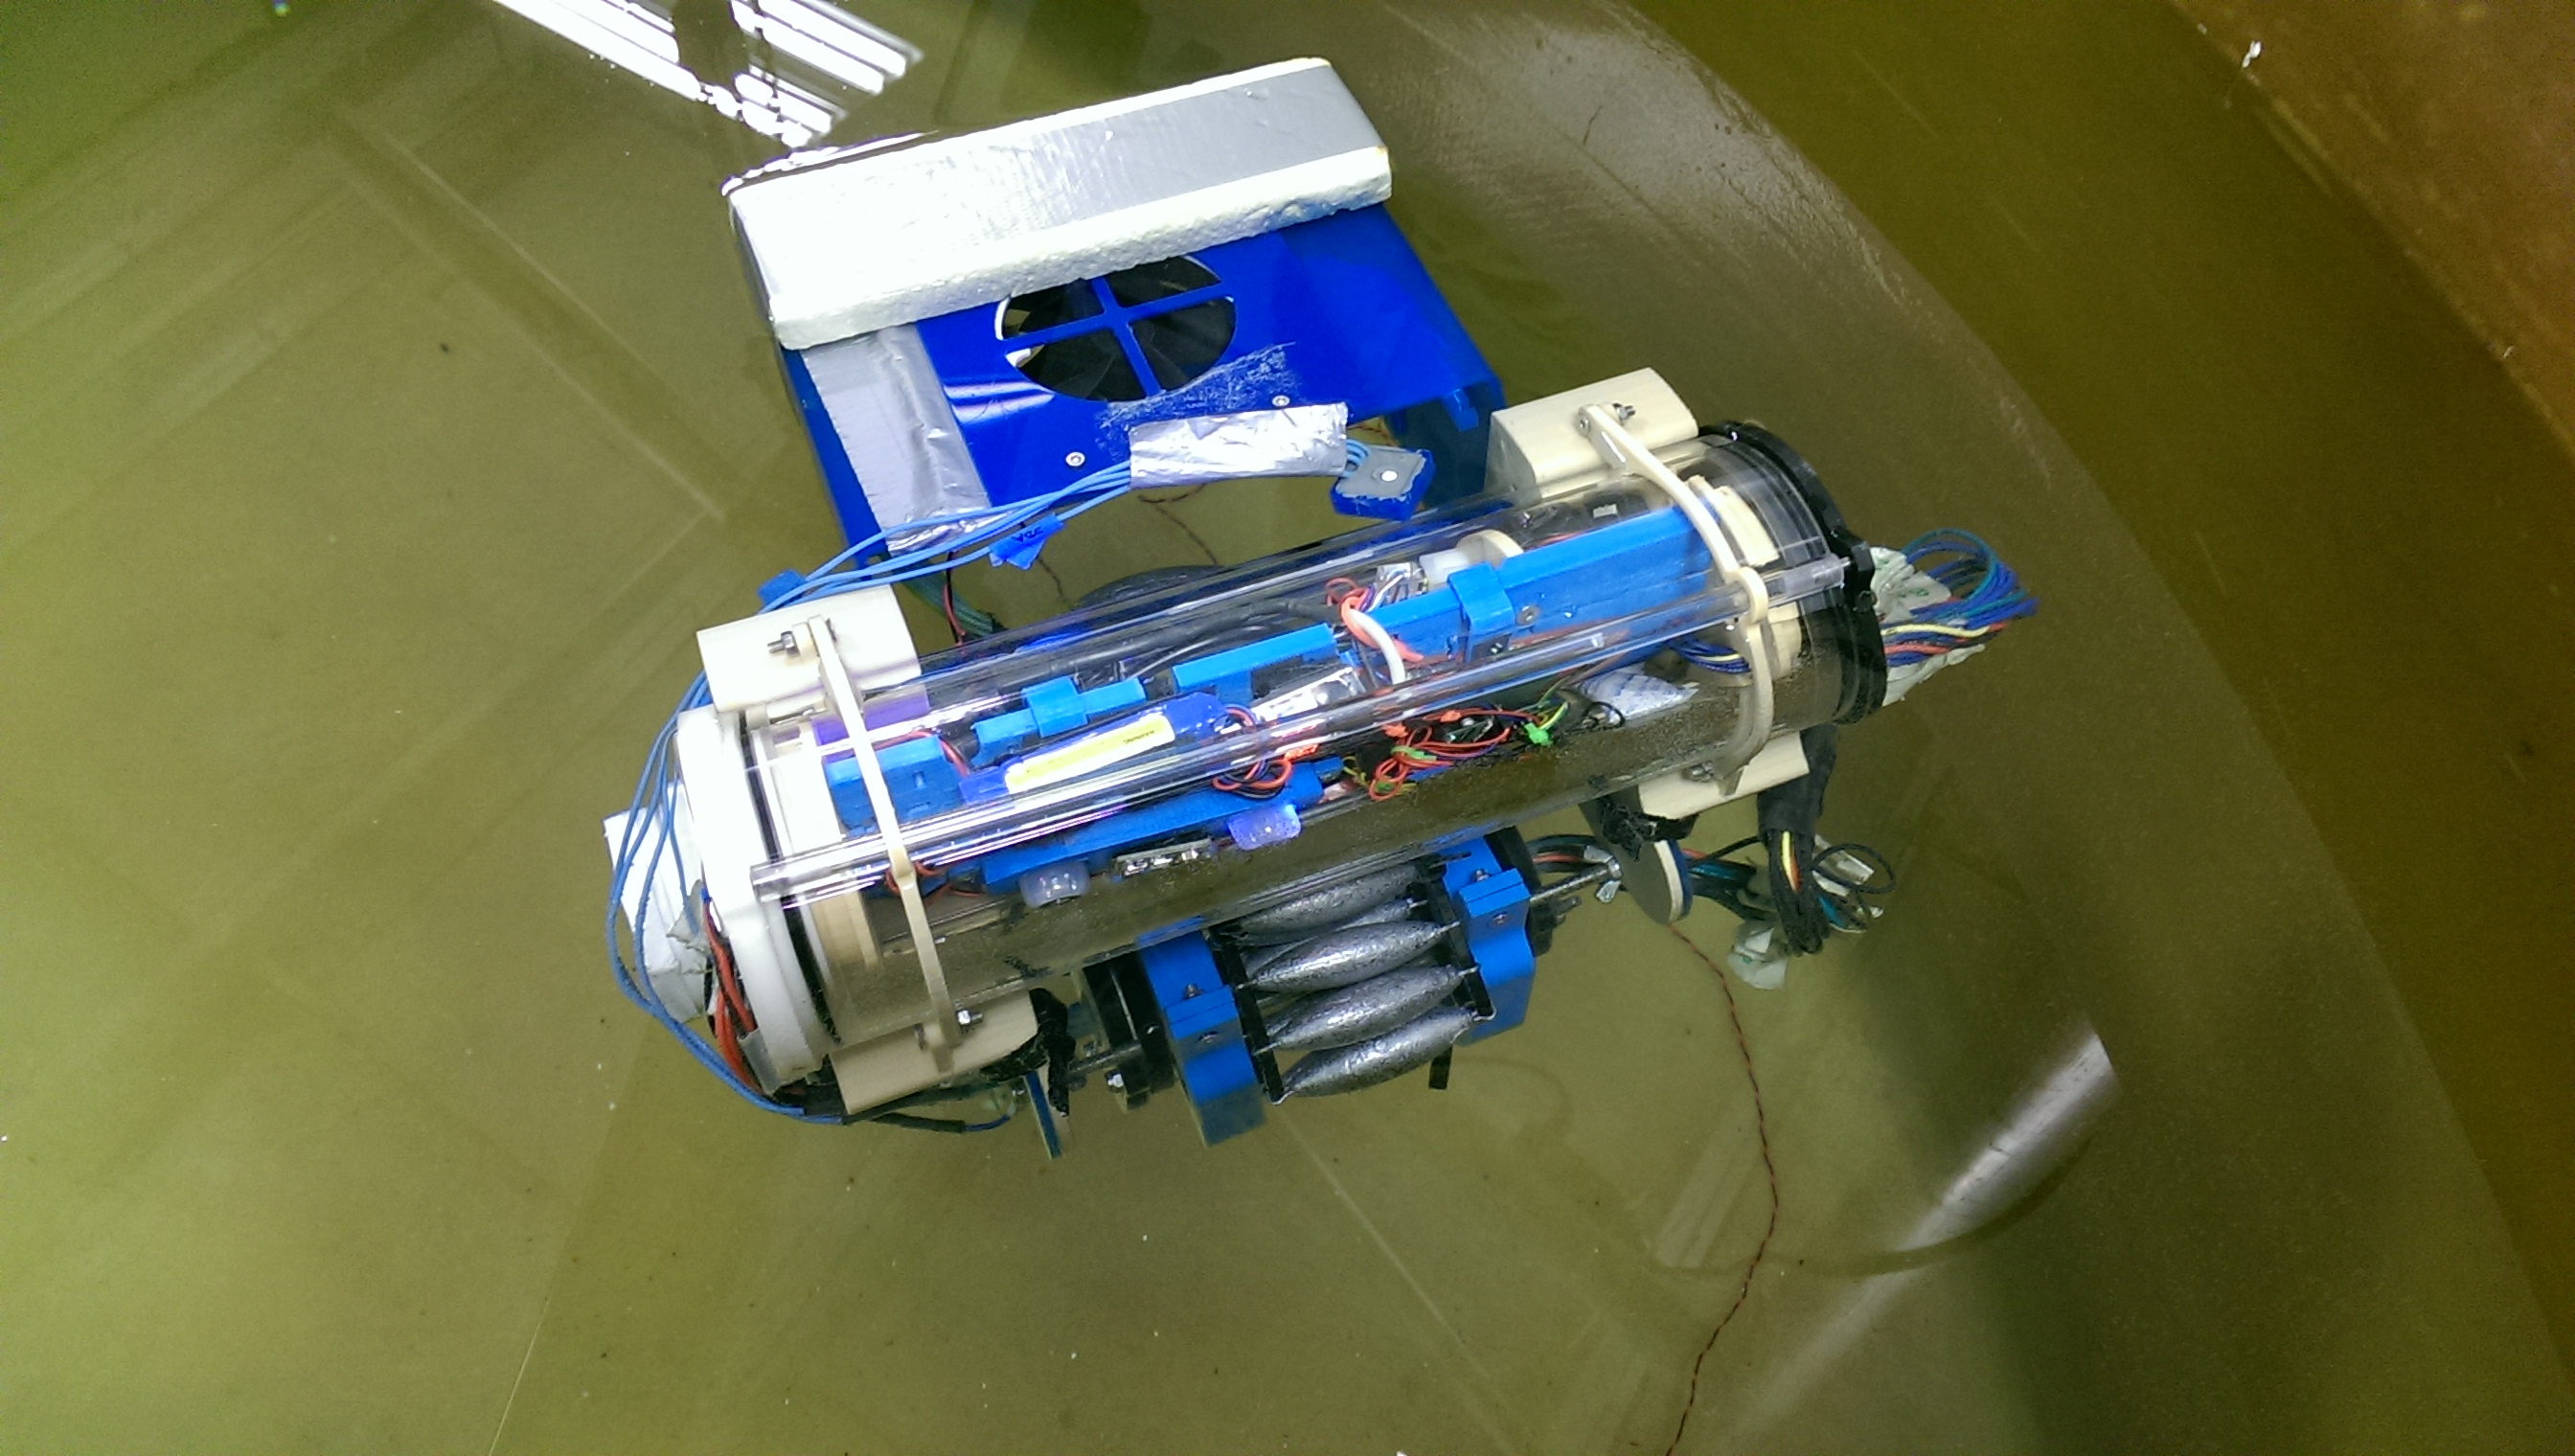
\includegraphics[width=0.45\textwidth]{cooprov_top.jpg}
      }
\caption{CoopROV shown in two different views}
\end{figure} 

\subsection{System Overview}

CoopROV is a \gls{rov} class submersible that is connected to a surface station through a tether. The surface station is a laptop computer. Both CoopROV and its surface station are connected by an ethernet interface and run a distributed \gls{ros} system. In teleoperation mode, a joystick controller connected to the surface station can drive the robot. The joystick controller can actuates the 3 thrusters (two at the back and one on top) offering the robot a 6-\gls{dof} motion. The robot is powered by two sets lithium ion batteries which can provide up to an hour of run time. A detailed accout of the different subsystems comprising hardware, electronics, software, sensors and power supply is discussed in the following sections.

\subsection{Hardware}

The exterior shell of CoopROV is composed of an acrylic frame that holds all housing tubes together. There are 3 housing tubes in total: the long transparent acrylic tube or the electronics tube, the short transparent acrylic tube or the connector tube and the pvc tube. There electronics tube holds all sensors and electronics of the robot. The connector housing tube has a connecter plug inside it. This connecter tube serves the purpose of a water proof connector plug that allows an easy way to swap sensor package of the \gls{rov} by simply plugging in and out a different electronics tube. There is also a PVC tube that holds the 11.1 V Li Ion batteries that power the motors of the robot. The clips and clamps that hold the tubes in place were made out of 3D-printed plastic parts. One big design improvement over OpenROV is the water proof seals that comprise a delrin end cap with an O-ring slot along with 3 threaded rods that maintain tension between the end cap and the acrylic tube. 

\subsection{Electronics}

\subsection{Power Supply}

\subsection{Sensors}

\subsection{Software}

\section{Test Infrastructure}

\section{Localization Experiments}

\section{Conclusion}

%========================================================================================
\printglossary[type=\acronymtype]                  
%
% This is the Bibliography file (bibtex.tex)
% This generally works for BibTeX

% Use sample.bib for BibTeX database
\bibliography{thesis_ref}
% BibTeX style (plain, alpha, unsrt)
\bibliographystyle{plain}
   % This file (bibtex.tex) contains the text
                   % for a bibliography if using BibTeX with
                   % sample.bib
\end{document}